\documentclass[12pt]{article}
\usepackage[utf8]{inputenc}
\usepackage[T1]{fontenc}
\usepackage{amsmath}
\usepackage{amsfonts}
\usepackage{amssymb}
\usepackage[version=4]{mhchem}
\usepackage{stmaryrd}
\usepackage{bbold}
\usepackage{physics}
\usepackage{graphicx}
\usepackage{subcaption}
\usepackage[export]{adjustbox}
\usepackage[a4paper, left=0.25in, right=0.25in, top=1in, bottom=1in]{geometry}
\graphicspath{ {./images/} }

\usepackage{listings} % Required for insertion of code
\usepackage{xcolor} % Required for custom colors

% Define custom colors
\definecolor{codegreen}{rgb}{0,0.6,0}
\definecolor{codegray}{rgb}{0.5,0.5,0.5}
\definecolor{codepurple}{rgb}{0.58,0,0.82}
\definecolor{backcolour}{rgb}{0.95,0.95,0.92}

% Setup the style for code listings
\lstdefinestyle{mystyle}{
    backgroundcolor=\color{backcolour},   
    commentstyle=\color{codegreen},
    keywordstyle=\color{magenta},
    numberstyle=\tiny\color{codegray},
    stringstyle=\color{codepurple},
    basicstyle=\ttfamily\footnotesize,
    breakatwhitespace=false,         
    breaklines=true,                 
    captionpos=b,                    
    keepspaces=true,                 
    numbers=left,                    
    numbersep=5pt,                  
    showspaces=false,                
    showstringspaces=false,
    showtabs=false,                  
    tabsize=2
}

% Activate the style
\lstset{style=mystyle}

\usepackage{hyperref}

\title{Assignment 4: Simulations with MPS }


\author{Instructor: Lesik Motrunich\\
TA: Liam O'Brien}
\date{}


%New command to display footnote whose markers will always be hidden
\let\svthefootnote\thefootnote
\newcommand\blfootnotetext[1]{%
  \let\thefootnote\relax\footnote{#1}%
  \addtocounter{footnote}{-1}%
  \let\thefootnote\svthefootnote%
}

%Overriding the \footnotetext command to hide the marker if its value is `0`
\let\svfootnotetext\footnotetext
\renewcommand\footnotetext[2][?]{%
  \if\relax#1\relax%
    \ifnum\value{footnote}=0\blfootnotetext{#2}\else\svfootnotetext{#2}\fi%
  \else%
    \if?#1\ifnum\value{footnote}=0\blfootnotetext{#2}\else\svfootnotetext{#2}\fi%
    \else\svfootnotetext[#1]{#2}\fi%
  \fi
}

\begin{document}
\maketitle
Due: $4 \mathrm{pm}$ Thursday, May 28,2024



\section*{4 Assignment: MPS simulations using TEBD}
We will again study the quantum Ising model subject to a magnetic field with both transverse and longitudinal components:


\begin{equation*}
H=-J \sum_{j=1}^{L-1} \sigma_{j}^{z} \sigma_{j+1}^{z}-h^{x} \sum_{j=1}^{L} \sigma_{j}^{x}-h^{z} \sum_{j=1}^{L} \sigma_{j}^{z} \tag{15}
\end{equation*}


Set $J=1$ and the magnetic field to $\left(h^{x}, h^{z}\right)=(-1.05,0.5)$, the same values as in Assignment 3, to allow you to test your MPS-based approach against exact diagonalization for small system sizes. Because we are now working with MPS, consider the system with open boundary conditions where the MPS simulations are most transparent. To specify a time-evolution procedure, this Hamiltonian can be arranged into three groups of commuting terms (i.e., commuting within each group): $H=H_{\text {odd }}+H_{\text {even }}+H_{\text {field }}$, each of which can be readily exponentiated. The groupings are


\begin{align*}
& H_{\mathrm{odd}}=-J \sum_{j=1,3,5, \ldots} \sigma_{j}^{z} \sigma_{j+1}^{z}=-J\left(\sigma_{1}^{z} \sigma_{2}^{z}+\sigma_{3}^{z} \sigma_{4}^{z}+\sigma_{5}^{z} \sigma_{6}^{z}+\cdots\right)  \tag{16}\\
& H_{\mathrm{even}}=-J \sum_{j=2,4,6, \ldots} \sigma_{j}^{z} \sigma_{j+1}^{z}=-J\left(\sigma_{2}^{z} \sigma_{3}^{z}+\sigma_{4}^{z} \sigma_{5}^{z}+\sigma_{6}^{z} \sigma_{7}^{z}+\cdots\right)  \tag{17}\\
& H_{\text {field }}=\sum_{j=1}^{L}\left(-h^{x} \sigma_{j}^{x}-h^{z} \sigma_{j}^{z}\right)=-h^{x} \sigma_{1}^{x}-h^{z} \sigma_{1}^{z}-h^{x} \sigma_{2}^{x}-h^{z} \sigma_{2}^{z}-h^{x} \sigma_{3}^{x}-h^{z} \sigma_{3}^{z}-\cdots \tag{18}
\end{align*}


Clearly the terms in $H_{\text {odd }}$ commute, and similarly for $H_{\text {even }}$, so they can be exponentiated directly:


\begin{equation*}
e^{-i t H_{\text {odd }}}=e^{i t J \sigma_{1}^{z} \sigma_{2}^{z}} e^{i t J \sigma_{3}^{z} \sigma_{4}^{z}} e^{i t J \sigma_{5}^{z} \sigma_{6}^{z}} \ldots, \quad e^{-i t H_{\text {even }}}=e^{i t J \sigma_{2}^{z} \sigma_{5}^{z}} e^{i t J \sigma_{4}^{z} \sigma_{5}^{\tilde{z}}} e^{i t J \sigma_{6}^{z} \sigma_{7}^{z}} \ldots \tag{19}
\end{equation*}


Within $H_{\text {field }}, \sigma_{j}^{x}$ and $\sigma_{j}^{z}$ do not commute on the same site. However, as these are single-site operators we can combine the terms for each $j$ into

\[
\omega_{j} \equiv-h^{x} \sigma_{j}^{x}-h^{z} \sigma_{j}^{z}=\left[\begin{array}{cc}
-h^{z} & -h^{x}  \tag{20}\\
-h^{x} & h^{z}
\end{array}\right]
\]

written in the $\sigma^{z}$ basis. As all of the $\omega_{j}$ commute, now $e^{-i t H_{\text {field }}}=e^{-i t \omega_{1}} e^{-i t \omega_{2}} e^{-i t \omega_{3}} \ldots$. Each $e^{-i t \omega_{j}}$ can be written out using formulas for Pauli matrices, e.g., $\exp (i \phi \boldsymbol{n} \cdot \boldsymbol{\sigma})=\cos (\phi)+i \sin (\phi) \boldsymbol{n} \cdot \boldsymbol{\sigma}$ [where $\boldsymbol{n}$ is a unit vector] for real time evolution, substituting hyperbolic functions for imaginary time evolution, or by direct exponentiation of the matrix. (Incidentally, you may notice that in this case other Trotter patterns than the one presented below are possible and may be more efficient. If you'd like, you can explore some of these, but the scheme outlined above will work regardless of the details of the terms in $H$.)

\subsection*{4.1 Imaginary time evolution}
"Rotate" now to imaginary time $\tau=i t$ and perform TEBD for cooling to the ground state. It will turn out that in this case all of the tensors are real-valued, but you should write your solution to also handle complex-valued tensors, for example using actual Hermitian conjugates rather than transposes; this will greatly simplify the process of going to real time evolution. However if your programming language is not strict about types, you may need to periodically cast complex values to reals in order to use specialized linear algebra routines.

First we will find the ground state of a small system, in order to compare with ED results. For $L=12$, create a simple ferromagnet state $|\psi(t=0)\rangle=|\uparrow\rangle \otimes|\uparrow\rangle \otimes|\uparrow\rangle \otimes \cdots$. As this is a product state, $\chi=1$ and all of the virtual indices take only one value: $a_{j}=\{1\}$. Set the $\left(A^{j}\right)_{a_{j-1}, a_{j}}^{\sigma_{j}}$ tensor components by hand; that is,


\begin{equation*}
\left(A^{1}\right)_{1}^{\uparrow}=1, \quad\left(A^{1}\right)_{1}^{\downarrow}=0 ; \quad\left(A^{2}\right)_{1,1}^{\uparrow}=1, \quad\left(A^{2}\right)_{1,1}^{\downarrow}=0 ; \text { etc. } \tag{21}
\end{equation*}


Because this state is unentangled, trivially it is already in canonical form for any site. As you operate with the Trotter gates generating entanglement between sites, the state will lose its canonical form. There is no need to work to restore it right away, because we will not truncate the virtual indices until applying all Trotter gates. To begin, measure the trial energy $E_{0}$ (i.e., expectation value of the Hamiltonian) of the initial state.

Exponentiate all local terms $h_{\alpha}$ to form the Trotter gates $e^{-\delta \tau h_{\alpha}}$ (a good starting value is $\delta \tau=\tau / n \sim 0.1$ ). Now apply the gates in the pattern (i) $e^{-\delta \tau H_{\text {field }}}$, (ii) $e^{-\delta \tau H_{\text {odd }}}$, (iii) $e^{-\delta \tau H_{\text {even }}}$, following the TEBD procedure in Sec. 3.2 . Notice that the single-site "gates" for $e^{-\delta \tau H_{\text {field }}}$ do not break the MPS form, thus for each $T_{j}=e^{-\delta \tau \omega_{j}}=\sum_{\sigma_{j}, \sigma_{j}} T_{\sigma_{j}^{\prime}}^{\sigma_{j}}\left|\sigma_{j}\right\rangle\left\langle\sigma_{j}^{\prime}\right|$ you can obtain the updated tensor without performing an SVD:


\begin{equation*}
\left(\tilde{A}^{j}\right)_{a_{j-1}, a_{j}}^{\sigma_{j}}=\sum_{\sigma_{j}^{\prime}} T_{\sigma_{j}^{\prime}}^{\sigma_{j}}\left(A^{j}\right)_{a_{j-1}, a_{j}}^{\sigma_{j}^{\prime}} \tag{22}
\end{equation*}


After applying all of the Trotter gates in this pattern we have a valid MPS, but the bond dimension will in general have grown. Using the method of Sec. 3.3, restore canonical form and truncate the MPS tensors using, say, $\chi=16$. This completes the process of taking the state from imaginary time 0 to $\delta \tau$. Use the canonical forms to perform an efficient measurement of the trial state energy $E_{\delta \tau}$ of the MPS. Then repeat the TEBD step above, measuring the energy at each time step. The state's convergence to the ground state can be determined from the change in the trial energy: set some tolerance $\varepsilon$ and check the condition $\left|E_{\tau}-E_{\tau-\delta \tau}\right| /\left|E_{\tau}\right|<\varepsilon$ to verify that the MPS has converged. Repeat the above for various increments $\delta \tau$; try for example $\delta \tau=0.1,0.01$, 0.001, and observe the effect on the converged energy. Compare with the true ground state energy of the Hamiltonian which you found using ED. Plot your trial energy for each $\delta \tau$ as a function of (imaginary) time along with the true ground state energy, and comment on the accuracy of the TEBD ground state\newpage
\begin{figure}
\begin{subfigure}{.5\textwidth}
  \centering
  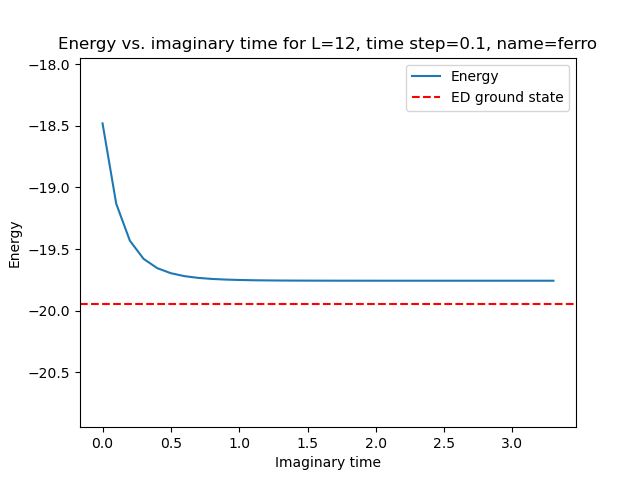
\includegraphics[width=\linewidth]{p4_1_energy_L_12_time_step_0.1_name_ferro.png}
\end{subfigure}
\begin{subfigure}{.5\textwidth}

    \centering
    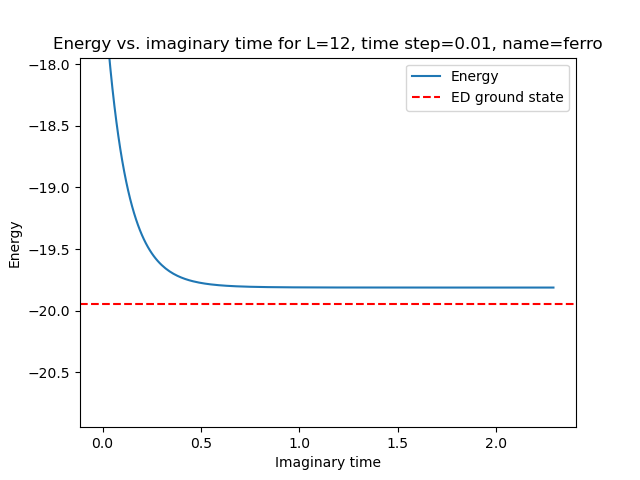
\includegraphics[width=\linewidth]{p4_1_energy_L_12_time_step_0.01_name_ferro.png}
\end{subfigure}
\end{figure}
\begin{figure}
\begin{subfigure}{.5\textwidth}
  \centering
  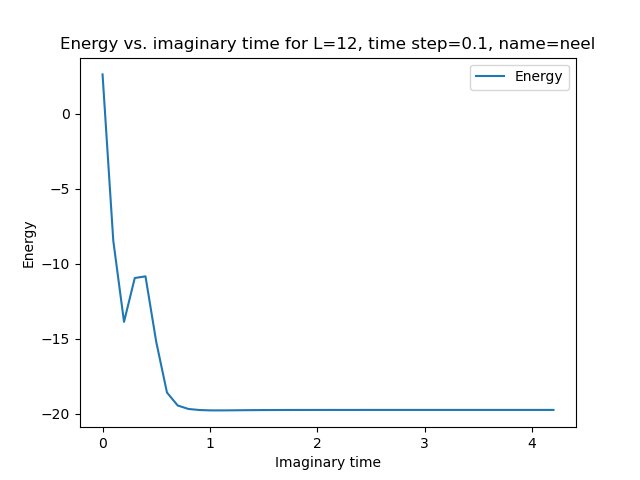
\includegraphics[width=\linewidth]{p4_1_energy_L_12_time_step_0.1_name_neel.png}
  \label{fig:2a}
\end{subfigure}
\begin{subfigure}{.5\textwidth}
  \centering
  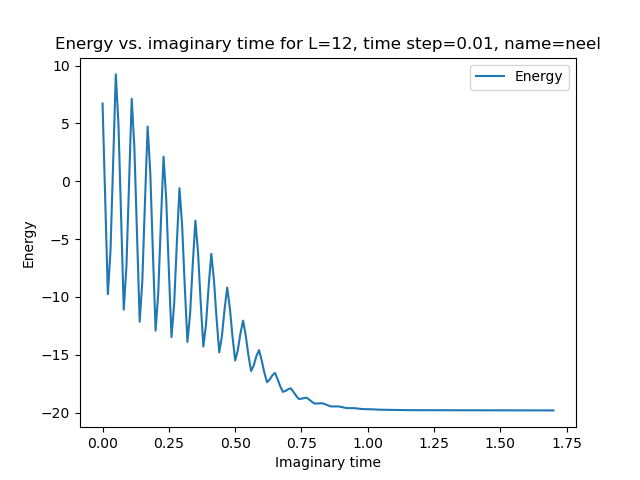
\includegraphics[width=\linewidth]{p4_1_energy_L_12_time_step_0.01_name_neel.png}
  \label{fig:2b}
\end{subfigure}

\end{figure}
As can be seen, an especially good approximation for the ground state is found using TEBD with imaginary time evolution. The simple ferromagnetic state is already fairly close to the ground state value, but Neel is not. For L=12, the initial trial energy was +9 for Neel, so it is noteworthy that such accurate results were able to be found at such a cheap computational cost. I should be observing that the imaginary time evolution causes exactly to the ground state, and this is why. First, let us consider the initial state in its decomposition:
\begin{equation}
  \ket{\psi _0} = \sum_{n} c_n \ket{\psi _n}
\end{equation}
which we then time evolved As
\begin{equation}
  \ket{\psi _t} = \sum_{n} c_n e^{-\tau E_n} \ket{\psi _n}
\end{equation}
Now, we divide by the normalization
\begin{equation}
  \frac{\sum_{n} c_n e^{-\tau E_n} \ket{\psi _n}}{\sqrt{|c_n|^2 e^{-2\tau E_n}}}
\end{equation}
In the denominator, we can factor out a ground state energy:
\begin{equation}
  \frac{\sum_{n} c_n e^{-\tau E_n} \ket{\psi _n}}{e^{-\tau E_0} \sqrt{|c_n|^2 e^{-2\tau (E_n - E_0)}}} = \frac{\sum_{n} c_n e^{-\tau (E_n - E_0)} \ket{\psi _n}}{\sqrt{|c_n|^2 e^{-2\tau (E_n - E_0)}}}
\end{equation}
So the exponent will be negative for any excited states and be strictly 0 for the ground state, so in theory, all excited states should be exponentially suppressed when we do the cooling process. My code almost achieves this, but not quite, and so we take the inner product of my final ground state with the true ground state, and see that in the sc it has matched the ground state almost correctly, but it is not absolute.
% Inline Python code in the document
\begin{lstlisting}[language=Python]
# compute the inner protect of this determined ground state with the true one from ed
tebd_gs = flatten_mps(ground_state)
inner_product = np.abs(np.vdot(tebd_gs, eigvecs[:, 0]))
                print(f'Inner product for {name} with L={L} and dt={dt} is {inner_product}')
def flatten_mps(mps):
    '''Flatten the MPS to remove all virtual indices.'''
    L = len(mps)
    combined = mps[0]

    # Sequentially contract the tensors
    for i in range(1, L-1):
        combined = np.einsum('...a,abc->...bc', combined, mps[i])

    # treat the final case wdifferently
    combined = np.einsum('...a,ab->...b', combined, mps[L-1])

    # Flatten the final combined tensor
    flattened_mps = combined.flatten()
    return flattened_mps()
\end{lstlisting}
\begin{figure}
  
\includegraphics{inner_p.png}
\end{figure}
% Inline Python code in the document
\begin{lstlisting}[language=Python]
import numpy as np
from hw2.src.p5_5 import truncate_svd
from scipy.linalg import expm
from hw4.src.contraction_fns import apply_local_hamiltonian
    
def create_trotter_gates(t, h_x=-1.05, h_z=0.5, J=1):
    """Create Trotter gates for the quantum Ising model."""
    # Define Pauli matrices
    sigma_x = np.array([[0, 1], [1, 0]])
    sigma_z = np.array([[1, 0], [0, -1]])

    # Single site Hamiltonian term
    omega = np.array([[-h_z, -h_x], [-h_x, h_z]])
    assert np.allclose(omega, omega.conj().T), "Omega is not Hermitian"
    
    # Interaction term
    interaction = -J * np.kron(sigma_z, sigma_z)
    assert np.allclose(interaction, interaction.conj().T), "Interaction is not Hermitian"
    
    # Create the Trotter gates
    gate_field = expm(1j * t * omega)
    # check whether this
    # assert np.allclose(gate_field.conj().T @ gate_field, np.eye(2))
    gate_odd = expm(1j * t * interaction).reshape(2, 2, 2, 2)
    # print(np.exp(1j * t * interaction))
    # assert np.allclose(gate_odd.conj().T @ gate_odd, np.eye(4))
    gate_even = gate_odd
    return gate_field, gate_odd, gate_even

def trotter_gate_field(mps, gate, site):
    """Apply a single Trotter gate to the MPS tensor at the given site."""
    mps_new = mps.copy()
    if site == 0:
        mps_new[site] = np.einsum('ik,ij->jk', mps[site], gate)
    elif site == len(mps) - 1:
        mps_new[site] = np.einsum('ij,ai->aj', gate, mps[site])
    else:
        mps_new[site] = np.einsum('ij,ajk->aik', gate, mps[site])
    return mps_new

def trotter_gate_interaction(mps, gate, site1, site2):
    """Apply a two-site Trotter gate to the MPS tensors at the given sites."""
    # make a copy of the mps tensors for modification
    mps_new = mps.copy()
    if site1 == 0:
        # Contract the first site with the gate
        w = np.einsum('ab,acdf,bfg->cdg', mps[site1], gate, mps[site2])
        w = w.reshape(gate.shape[1], gate.shape[2]*mps[site2].shape[2])
        # compute the SVD
        U, S, V = np.linalg.svd(w, full_matrices=False)
        # Update the MPS tensors
        mps_new[site1] = U.reshape(2, -1)
        mps_new[site2] = (np.diag(S) @ V).reshape(-1, 2, mps[site2].shape[2])
    elif site2 == len(mps) - 1:
        # Contract the last site with the gate
        w = np.einsum('abc,bdfg,cg->adf', mps[site1], gate, mps[site2])
        w = w.reshape(mps[site1].shape[0]*gate.shape[1], gate.shape[3])
        # compute the SVD
        U, S, V = np.linalg.svd(w, full_matrices=False)
        # Update the MPS tensors
        mps_new[site1] = U.reshape(mps[site1].shape[0], 2, -1)
        mps_new[site2] = (np.diag(S) @ V).reshape(-1, 2)
    else:
        w = np.einsum('abc,befd,cdg->aefg', mps[site1], gate, mps[site2])
        w = w.reshape(mps[site1].shape[0]*gate.shape[1], gate.shape[2]*mps[site2].shape[2])
        # compute the SVD
        U, S, V = np.linalg.svd(w, full_matrices=False)
        # Update the MPS tensors
        mps_new[site1] = U.reshape(mps[site1].shape[0], 2, -1)
        mps_new[site2] = (np.diag(S) @ V).reshape(-1, 2, mps[site2].shape[2])
    return mps_new

def apply_trotter_gates(mps, gate_field, gate_odd, gate_even):
    """Apply Trotter gates to the entire MPS."""
    L = len(mps)
    # Apply field gates
    # verify that the gate is unitary
    # assert np.allclose(gate_field.conj().T @ gate_field, np.eye(2))
    # Apply field gates
    for i in range(L):
        mps = trotter_gate_field(mps, gate_field, i)
    # Apply odd interaction gates
    for i in range(0, L-1, 2):
        mps = trotter_gate_interaction(mps, gate_odd, i, i+1)
    
    # Apply even interaction gates
    for i in range(1, L-1, 2):
        mps = trotter_gate_interaction(mps, gate_even, i, i+1)
    
    return mps

def check_left_canonical(tensor):
        left_canonical = False 
        if len(tensor.shape) == 2:
            tensor = tensor.reshape(1, *tensor.shape)
        if np.allclose(np.einsum('ijk,kjm->im' , tensor.conj().T, tensor), np.eye(tensor.shape[2])):
            left_canonical = True
        return left_canonical

def check_right_canonical(tensor):
    right_canonical = False
    if len(tensor.shape) == 2:
        tensor = tensor.reshape(*tensor.shape, 1)
    if np.allclose(np.einsum('ijk,kjm->im' , tensor, tensor.conj().T), np.eye(tensor.shape[0])):
        right_canonical = True
    return right_canonical
            
def enforce_bond_dimension(mps, chi):
    """Enforce left and right canonical forms on the MPS without truncating."""
    L = len(mps)
    
    # Left-to-right sweep
    for i in range(L-1):
        if i == 0:
            contraction = np.einsum('ij,jab->iab', mps[i], mps[i+1])
            w = contraction.reshape(mps[i].shape[0], mps[i+1].shape[1]*mps[i+1].shape[2])
            U, S, V = np.linalg.svd(w, full_matrices=False)
            mps[i] = U.reshape(mps[i].shape[0], -1)
            assert check_left_canonical(mps[i])
            mps[i+1] = (np.diag(S) @ V).reshape(-1, mps[i+1].shape[1], mps[i+1].shape[2])
        elif i == L-2:
            contraction = np.einsum('ijk,kl->ijl', mps[i], mps[i+1])
            w = contraction.reshape(mps[i].shape[0]*mps[i].shape[1], mps[i+1].shape[1])
            U, S, V = np.linalg.svd(w, full_matrices=False)

            s = S/np.sqrt(np.sum(np.diag(S) ** 2))
            
            mps[i] = U.reshape(mps[i].shape[0], mps[i].shape[1], -1)
            assert check_left_canonical(mps[i])
            mps[i+1] = (np.diag(s) @ V).reshape(-1, mps[i+1].shape[1])
            assert not check_left_canonical(mps[i+1])
        else:
            contraction = np.einsum('ijk,klm->ijlm', mps[i], mps[i+1])
            w = contraction.reshape(mps[i].shape[0]*mps[i].shape[1], mps[i+1].shape[1]*mps[i+1].shape[2])
            U, S, V = np.linalg.svd(w, full_matrices=False)
            mps[i] = U.reshape(mps[i].shape[0], mps[i].shape[1], -1)
            assert check_left_canonical(mps[i])
            mps[i+1] = (np.diag(S) @ V).reshape(-1, mps[i+1].shape[1], mps[i+1].shape[2])

    # Right-to-left sweep
    for i in range(L-1, 0, -1):
        if i == L-1:
            contraction = np.einsum('ijk,kl->ijl', mps[i-1], mps[i])
            w = contraction.reshape(mps[i-1].shape[0]*mps[i-1].shape[1], mps[i].shape[1])
            u, s_diag, vt = truncate_svd(w, chi)
            mps[i-1] = (u @ s_diag).reshape(mps[i-1].shape[0], mps[i-1].shape[1], -1)
            mps[i] = vt.reshape(-1, mps[i].shape[1])
            assert check_right_canonical(mps[i])
        elif i == 1:
            contraction = np.einsum('ai,ijk->ajk', mps[i-1], mps[i])
            w = contraction.reshape(mps[i-1].shape[0], mps[i].shape[1]*mps[i].shape[2])
            u, s_diag, vt = truncate_svd(w, chi)
            mps[i-1] = (u @ s_diag).reshape(-1, mps[i].shape[0])
            mps[i] = vt.reshape(mps[i].shape[0], mps[i].shape[1], -1)
            assert check_right_canonical(mps[i])
        else:
            contraction = np.einsum('ijk,klm->ijlm', mps[i-1], mps[i])
            w = contraction.reshape(mps[i-1].shape[0]*mps[i-1].shape[1], mps[i].shape[1]*mps[i].shape[2])
            u, s_diag, vt = truncate_svd(w, chi)
            mps[i-1] = (u @ s_diag).reshape(mps[i-1].shape[0], mps[i-1].shape[1], -1)
            mps[i] = vt.reshape(-1, mps[i].shape[1], mps[i].shape[2])
            assert check_right_canonical(mps[i])
    
    return mps

def create_initial_mps(l, name):
    up_physical = np.array([1, 0])
    down_physical = np.array([0, 1])
    single_sight = np.array([1, -np.sqrt(3)]) / 2 
    mps = []
    for i in range(l):
        if i == 0:
            up_reshape = up_physical.reshape(2, 1)
            if name == 'ferro' or name == 'neel':
                mps.append(up_reshape)
            elif name == 'three':
                mps.append(single_sight.reshape(2, 1))
        elif i == l-1:
            up_reshape = up_physical.reshape(1, 2)
            down_reshape = down_physical.reshape(1, 2)
            if name == 'ferro':
                mps.append(up_reshape)
            elif name == 'neel':
                mps.append(up_reshape if i % 2 == 0 else down_reshape)
            elif name == 'three':
                mps.append(single_sight.reshape(1, 2))
        else:
            up_reshape = up_physical.reshape(1, 2, 1)
            down_reshape = down_physical.reshape(1, 2, 1)
            if name == 'ferro':
                mps.append(up_reshape)
            elif name == 'neel':
                mps.append(up_reshape if i % 2 == 0 else down_reshape)
            elif name == 'three':
                mps.append(single_sight.reshape(1, 2, 1))
    return mps

# make a function that will get red of all of the virtual indices to just leave the physical indices of an mps
def flatten_mps(mps):
    '''Flatten the MPS to remove all virtual indices.'''
    L = len(mps)
    combined = mps[0]

    # Sequentially contract the tensors
    for i in range(1, L-1):
        combined = np.einsum('...a,abc->...bc', combined, mps[i])

    # treat the final case wdifferently
    combined = np.einsum('...a,ab->...b', combined, mps[L-1])

    # Flatten the final combined tensor
    flattened_mps = combined.flatten()
    return flattened_mps

def imaginary_tebd_step(current_mps, chi, time, gates):
    """Imaginary time evolution using TEBD."""
    gate_field, gate_odd, gate_even = gates
    trotterized = apply_trotter_gates(current_mps, gate_field, gate_odd, gate_even)
    mps_enforced = enforce_bond_dimension(trotterized, chi)
    return mps_enforced
import numpy as np
import matplotlib.pyplot as plt

from hw4.src.p4_1.imaginary_tebd_fns import create_trotter_gates, apply_trotter_gates, enforce_bond_dimension, create_initial_mps, flatten_mps
from hw4.src.contraction_fns import apply_local_hamiltonian, compute_contraction
from hw4.src.p4_1.ed_fns import open_dense_hamiltonian
from hw4.src.p4_1.plt_fns import plot_energy_vs_time, plot_ground_state_density, get_correlations, plot_correlations





def main():
    H = open_dense_hamiltonian(8)
    eigvals, eigvecs = np.linalg.eigh(H)
    gs_e_12 = eigvals[0]
    system_sizes = [8]
    total_time = 8
    time_steps = [0.01]
    initial_states = ['ferro', 'neel']
    chi = 10

    ground_states = {}
    ground_state_energies = {}

    for name in initial_states:
        ground_states[name] = {}
        ground_state_energies[name] = {}
        
        for L in system_sizes:
            if L == 12 and name == 'ferro':
                gs_e = gs_e_12
            else:
                gs_e = None
            ground_states[name][L] = {}
            ground_state_energies[name][L] = {}
            
            for dt in time_steps:
                ground_state, energies = compute_ground_state(L, chi, total_time, dt, name)
                ground_states[name][L][dt] = ground_state
                # compute the inner protect of this determined ground state with the true one from ed
                tebd_gs = flatten_mps(ground_state)
                
                inner_product = np.abs(np.vdot(tebd_gs, eigvecs[:, 0]))
                print(f'Inner product for {name} with L={L} and dt={dt} is {inner_product}')
                
                ground_state_energies[name][L][dt] = energies
                
                plot_energy_vs_time(energies, name, L, dt, gs_e)
        
        plot_ground_state_density(ground_state_energies[name], name)
        # only measure the correlations for the largest system size in the list
        for L in system_sizes[-1:]:
            # also do this only for the small list time step coma which is at the end of the list
            for dt in time_steps[-1:]:
                correlations = get_correlations(ground_states[name][L][dt])
                plot_correlations(correlations, name, L, dt)

if __name__ == "__main__":
    main()
 

    

        
    
    

        
    
    
\end{lstlisting}
\newpage

Now we no longer need to restrict to small system sizes. You can find the ground states for larger systems, like $L=32,64,128$. \textbf{Either because of my computer, the language, or a slow implementation, I was not able to get up to the large system sizes suggested, but I try to do things that I could not do with ED throughout.}(If the bond dimension is kept fixed, which is suitable for ground states with finite entanglement, the computational cost grows roughly linearly with $L$ and is very manageable.) Plot the convergence of the ground state energy density, which is the extrapolation to $L \rightarrow \infty$, using the quantity $(E(L+x)-E(L)) / x$ for consecutive system sizes (you used this method in Assignment 1 to mitigate finite size effects for open boundary conditions, which is also the case here). Using the converged ground states, also measure some correlation functions in large systems. \textbf{Even though my correlation functions are kind of wacky, which might stem from the fact that I have not actually called to the ground state, we can see that the neel and ferro have the same plots because we cool to the same ground state with any initial state.}
\begin{figure}[h!]
  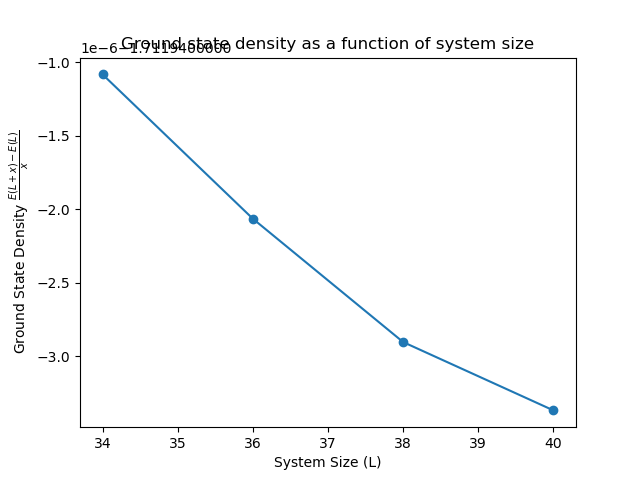
\includegraphics[width=0.4\textwidth]{ground_state_density_tst.png}
\end{figure}
\begin{figure}[h!]
  \centering
  \begin{subfigure}[b]{0.4\textwidth}
    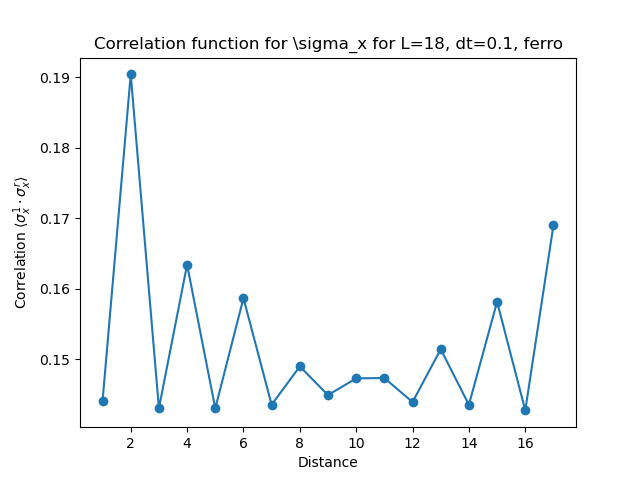
\includegraphics[width=\textwidth]{p4_1_correlation_sigma_x_L_18_dt_0.1_name_ferro.png}
    \caption{Ferro - $\sigma_x$}
  \end{subfigure}
  \hfill
  \begin{subfigure}[b]{0.4\textwidth}
    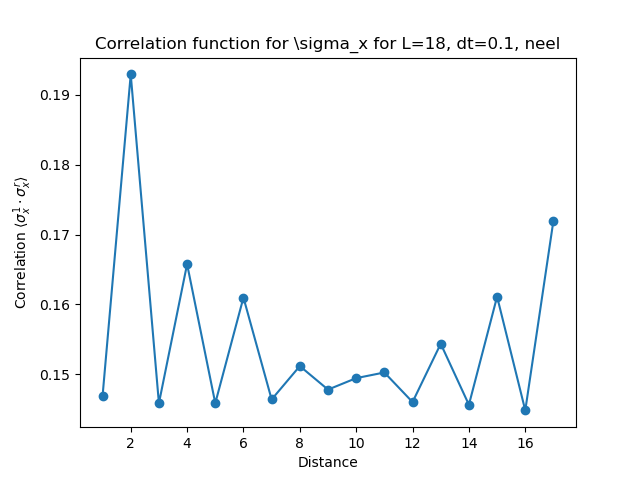
\includegraphics[width=\textwidth]{p4_1_correlation_sigma_x_L_18_dt_0.1_name_neel.png}
    \caption{Neel - $\sigma_x$}
  \end{subfigure}
  \caption{Correlation function for $\sigma_x$}
\end{figure}

\begin{figure}[h!]
  \centering
  \begin{subfigure}[b]{0.4\textwidth}
    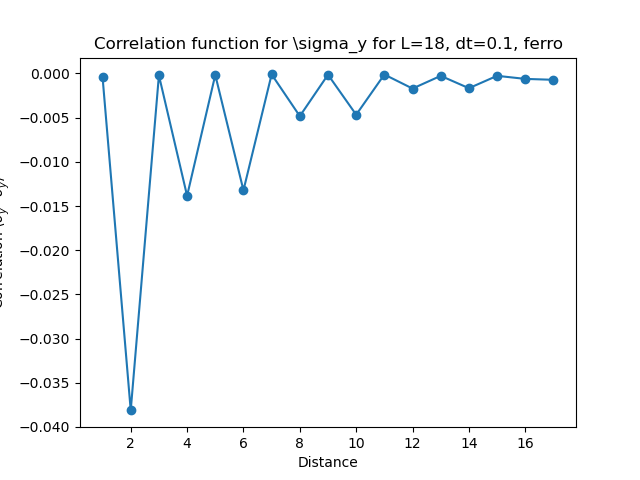
\includegraphics[width=\textwidth]{p4_1_correlation_sigma_y_L_18_dt_0.1_name_ferro.png}
    \caption{Ferro - $\sigma_y$}
  \end{subfigure}
  \hfill
  \begin{subfigure}[b]{0.4\textwidth}
    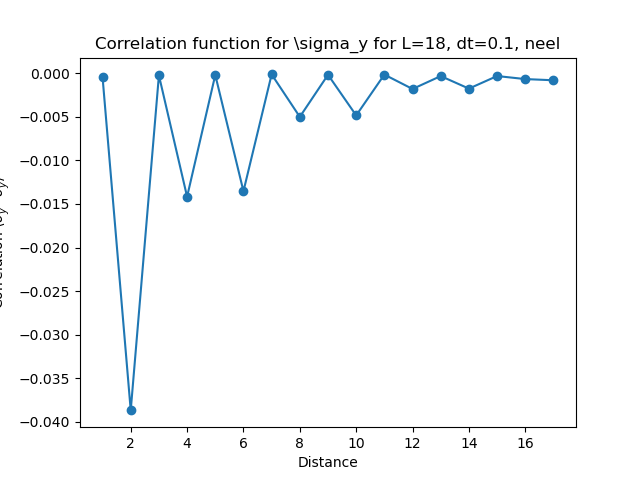
\includegraphics[width=\textwidth]{p4_1_correlation_sigma_y_L_18_dt_0.1_name_neel.png}
    \caption{Neel - $\sigma_y$}
  \end{subfigure}
  \caption{Correlation function for $\sigma_y$}
\end{figure}

\begin{figure}[h!]
  \centering
  \begin{subfigure}[b]{0.4\textwidth}
    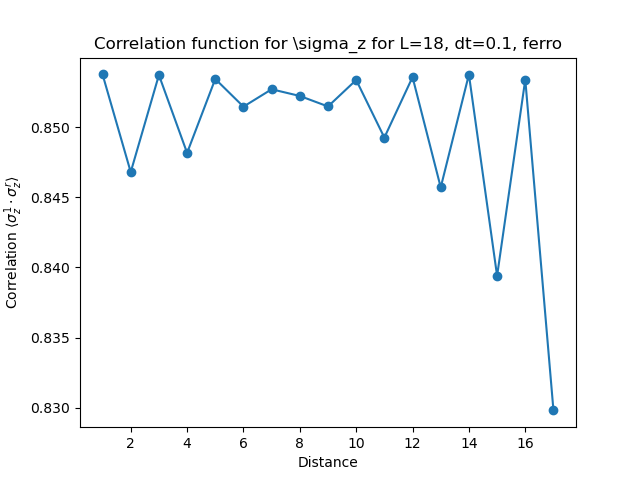
\includegraphics[width=\textwidth]{p4_1_correlation_sigma_z_L_18_dt_0.1_name_ferro.png}
    \caption{Ferro - $\sigma_z$}
  \end{subfigure}
  \hfill
  \begin{subfigure}[b]{0.4\textwidth}
    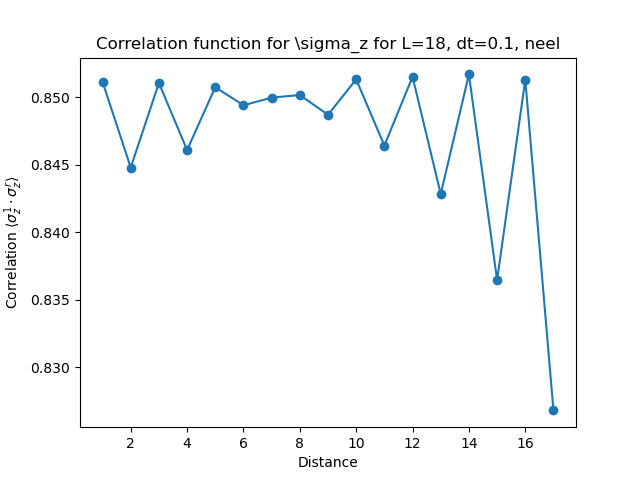
\includegraphics[width=\textwidth]{p4_1_correlation_sigma_z_L_18_dt_0.1_name_neel.png}
    \caption{Neel - $\sigma_z$}
  \end{subfigure}
  \caption{Correlation function for $\sigma_z$}
\end{figure}
% Inline Python code in the document
\begin{lstlisting}[language=Python]
# only measure the correlations for the largest system size in the list
        for L in system_sizes[-1:]:
            # also do this only for the small list time step coma which is at the end of the list
            for dt in time_steps[-1:]:
                correlations = get_correlations(ground_states[name][L][dt])
                plot_correlations(correlations, name, L, dt)

def get_correlations(mps):
    L = len(mps)
    correlations = {}
    sigma_x = np.array([[0, 1], [1, 0]])
    sigma_y = np.array([[0, -1j], [1j, 0]])
    sigma_z = np.array([[1, 0], [0, -1]])
    sigmas = [sigma_x, sigma_y, sigma_z]

    for s, sigma in enumerate(sigmas):
        correlations[s] = {}
        first_tensor = mps[0]
        first_sigma_contraction = np.einsum('bc,bd,de->ce', first_tensor.conj(), sigma, first_tensor)
        
        for i in range(1, L):
            second_tensor = mps[i]
            if i == L-1:
                second_sigma_contraction = np.einsum('ab,bd,cd->ac', second_tensor.conj(), sigma, second_tensor)
            else:
                second_sigma_contraction = np.einsum('abc,bd,jdc->aj', second_tensor.conj(), sigma, second_tensor)
            
            for j in range(i-1, 0, -1):
                second_sigma_contraction = np.einsum('akc,jkl,cl->aj', mps[j].conj(), mps[j], second_sigma_contraction)
            
            correlations[s][i] = np.einsum('ab,ab->', first_sigma_contraction, second_sigma_contraction)

    return correlations
\end{lstlisting}





Finally, for a fixed (large) system size, study the convergence of an initial product state with a Néel pattern $|\psi(t=0)\rangle=|\uparrow\rangle \otimes|\downarrow\rangle \otimes|\uparrow\rangle \otimes|\downarrow\rangle \otimes \cdots$, including showing the trial energy as the state cools and also measuring some correlations in the converged state. Compare to the results you found using the ferromagnetic initial state.\\
\textbf{This was explained earlier.}
\newpage

\subsection*{4.2 Real time evolution: quench dynamics}
Rotate back to perform real time evolution: $\tau \rightarrow i t$. The gates and MPS tensors will now generally be complex-valued, but this should require little modification to your solution from the previous\\
section. You may need to be careful here if your linear algebra routines are specialized to realvalued matrices, as you would need to switch to complex-valued routines here. If your linear algebra package figures out types automatically, you will likely not need to change the call to your diagonalization routine, but be careful to use Hermitian conjugation where required instead of matrix transpose, as these are different operations. Again choose $\delta t$ small, and use a fairly large system size $L$ (you can try multiple options). First we will study a quantum quench problem, timeevolving an arbitrary state under the Hamiltonian (15). Use the product state from the previous assignment:


\begin{equation*}
|\psi(t=0)\rangle=|\xi\rangle_{1} \otimes|\xi\rangle_{2} \otimes \cdots \otimes|\xi\rangle_{L}, \quad|\xi\rangle=\frac{1}{2}(|\uparrow\rangle-\sqrt{3}|\downarrow\rangle) \tag{23}
\end{equation*}


Encode this state as an MPS by setting the tensor components by hand. Measure some observables,

like $\left\langle\sigma_{L / 2}^{x}\right\rangle,\left\langle\sigma_{1}^{x}\right\rangle,\left\langle\sigma_{L / 2}^{z}\right\rangle$, etc., in the initial state and during the evolution. Note that the system Hamiltonian is not translation invariant because of the boundaries, and the same observables on different sites may differ at nonzero time.\\


\begin{figure}[h!]
  \centering
  \begin{subfigure}[b]{0.48\textwidth}
    \centering
    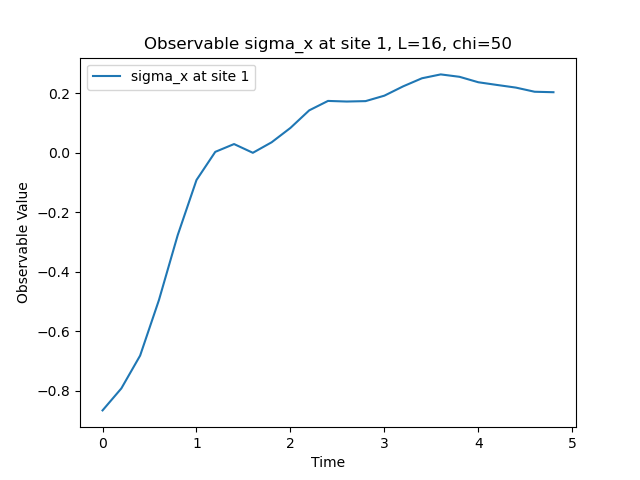
\includegraphics[width=\textwidth]{observable_sigma_x_site_1_L_16_chi_50.png}
    \caption{$\sigma_x$ at site 1, L=16, $\chi$=50}
  \end{subfigure}
  \hfill
  \begin{subfigure}[b]{0.48\textwidth}
    \centering
    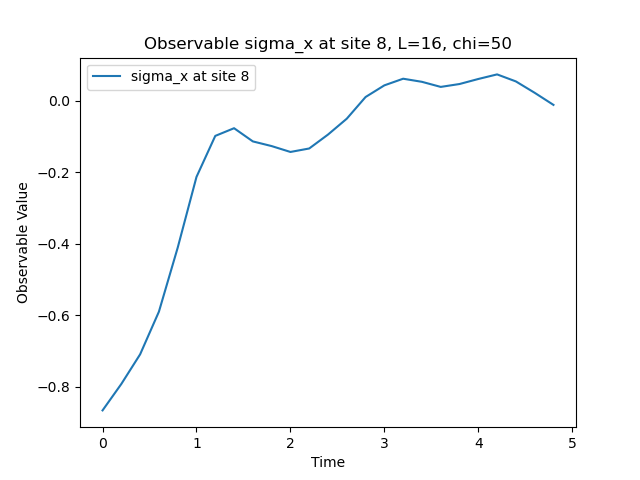
\includegraphics[width=\textwidth]{observable_sigma_x_site_8_L_16_chi_50.png}
  \end{subfigure}
  
  \begin{subfigure}[b]{0.48\textwidth}
    \centering
    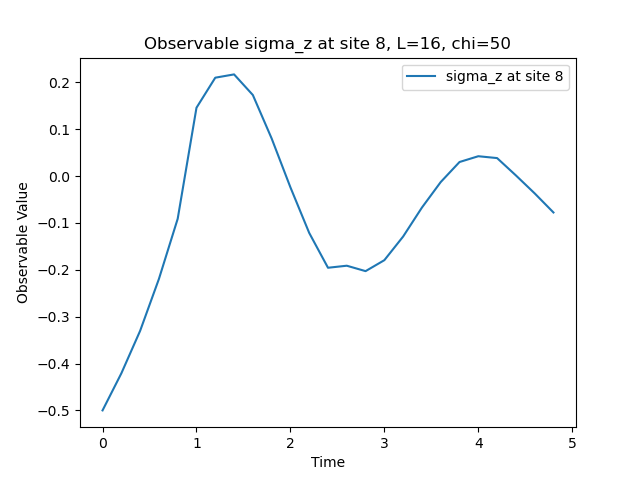
\includegraphics[width=\textwidth]{observable_sigma_z_site_8_L_16_chi_50.png}
    \caption{$\sigma_z$ at site 8, L=16, $\chi$=50}
  \end{subfigure}
  
  \caption{Observables for different $\sigma$ values, sites, and system sizes}
\end{figure}
% Inline Python code in the document
\begin{lstlisting}[language=Python]
def real_tebd(L, chi, total_time, dt, name):
    """Real time evolution using TEBD."""
    initial_mps = create_initial_mps(L, name)
    # measure some observables of the initial state
    first_observable = ('sigma_x', int(L/2))
    second_observable = ('sigma_x', 1)
    third_observable = ('sigma_z', int(L/2))
    observables = [first_observable, second_observable, third_observable]
    observable_values = {obs: {} for obs in observables}

    times = np.arange(0, total_time, dt)
    energies = {}
    entropies = {}
    current_mps = initial_mps
    gate_field, gate_odd, gate_even = create_trotter_gates(-dt)

    for time in times:
        for observable in observables:
            observable_values[observable][time] = measure_observable(current_mps, observable[0], observable[1])
        # compute the entitlement and copy for the half system
        ee = entanglement_entropy(current_mps, int(L/2))
        entropies[time] = ee
        trotterized = apply_trotter_gates(current_mps, gate_field, gate_odd, gate_even)
        mps_enforced = enforce_bond_dimension(trotterized, chi)
        energy = apply_local_hamiltonian(mps_enforced)
        print(f'Energy at time {time} is {energy}')

        energies[time] = energy

        if time > 0:
            prev_time = time - dt
            if prev_time in energies and (np.abs(energy - energies[prev_time]) / np.abs(energy)) < 1e-8:
                final_gs = mps_enforced
                break

        current_mps = mps_enforced

    return observable_values, entropies, times

def plot_observables(observable_values, L, chi):
    for observable, values in observable_values.items():
        times_sorted = sorted(values.keys())
        values_sorted = [values[time] for time in times_sorted]
        
        plt.figure()
        plt.plot(times_sorted, values_sorted, label=f'{observable[0]} at site {observable[1]}')
        plt.xlabel('Time')
        plt.ylabel('Observable Value')
        plt.title(f'Observable {observable[0]} at site {observable[1]}, L={L}, chi={chi}')
        plt.legend()
        plt.savefig(f"hw4/docs/images/observable_{observable[0]}_site_{observable[1]}_L_{L}_chi_{chi}.png")
    return
\end{lstlisting}

\newpage
Use TEBD to evolve in real time, measuring observables after every time step. 
\begin{figure}
  
\end{figure}
Here again you may want to check your new MPS-based method against ED simulations for a small chain and short times (modifying your code from Assignment 3 to open boundary conditions), before doing more exploratory studies in what follows. Choose a maximum bond dimension (say, $\chi=16$) and also measure the half-system entanglement entropy $S_{L/2}$ at every time step. You should observe that, in contrast to the imaginary-time case, the EE grows until it reaches the largest value supported by the MPS, then saturates. Once this happens we cannot trust the results of TEBD any longer; this is an important barrier to studying dynamics in large quantum systems. Repeat the experiment with larger $\chi=64,128$ and see what times you can reach with reliable results. Try a different initial state to verify that the entanglement growth is not atypical; plot all of the entanglement entropies $S_{L/2}$ you have measured. Can you detect the saturation point (where the dynamics becomes nonphysical) in the time traces of the observables?

\begin{figure}[h!]
  \centering
  \begin{subfigure}[b]{0.48\textwidth}
    \centering
    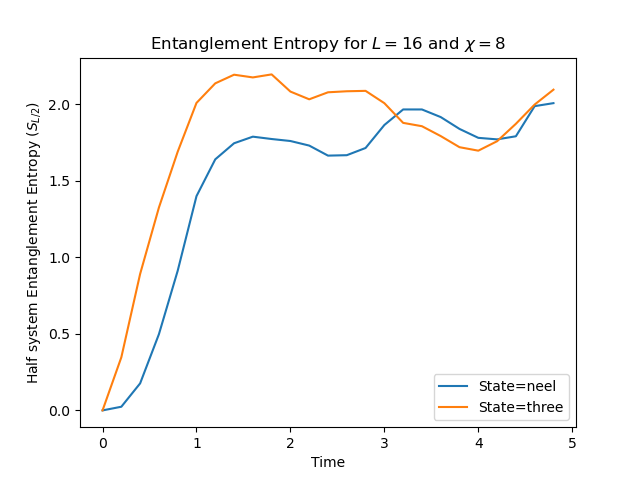
\includegraphics[width=\textwidth]{combined_hs_ee_L_16_chi_8.png}
    \caption{L=16, $\chi$=8}
  \end{subfigure}
  \hfill
  \begin{subfigure}[b]{0.48\textwidth}
    \centering
    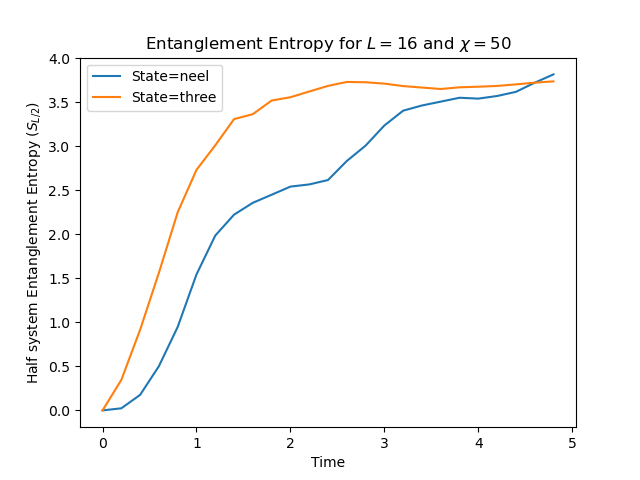
\includegraphics[width=\textwidth]{combined_hs_ee_L_16_chi_50.png}
    \caption{L=16, $\chi$=50}
  \end{subfigure}
  
  \caption{Combined HS and EE for different $\chi$ values at L=16}
\end{figure}
As seen in these figures, the lower entanglement entropy saturates earlier (at about a time of 1.5), while the higher $\chi$ saturates at a much later time of about 4. The reason for this difference is that we chose different values for $\chi$, and the virtual bond dimension is a measure of the limit of how much information can be contained within the MPS. This is why, for the case of $\chi=8$, it is not only that the entanglement entropy saturates much earlier than for the other case, but the magnitude of this entanglement entropy is in general lower, because we have contained less information with the smaller bond dimension. One can determine this saturation point wherever the curve "levels off" and the entanglement entropy no longer grows.
% Inline Python code in the document
\begin{lstlisting}[language=Python]
import numpy as np
import matplotlib.pyplot as plt
from hw4.src.p4_1.ed_fns import open_dense_hamiltonian
from hw4.src.p4_1.imaginary_tebd_fns import create_initial_mps, create_trotter_gates, apply_trotter_gates, enforce_bond_dimension
from hw4.src.contraction_fns import apply_local_hamiltonian
from hw4.src.p4_2.observable_fns import measure_observable, plot_observables, entanglement_entropy, plot_entanglement_entropy, plot_combined_entanglement_entropy
from hw4.src.p4_3.dynamics_fns import apply_observable

def real_tebd(L, chi, total_time, dt, name):
    """Real time evolution using TEBD."""
    initial_mps = create_initial_mps(L, name)
    # measure some observables of the initial state
    first_observable = ('sigma_x', int(L/2))
    second_observable = ('sigma_x', 1)
    third_observable = ('sigma_z', int(L/2))
    observables = [first_observable, second_observable, third_observable]
    observable_values = {obs: {} for obs in observables}

    times = np.arange(0, total_time, dt)
    energies = {}
    entropies = {}
    current_mps = initial_mps
    gate_field, gate_odd, gate_even = create_trotter_gates(-dt)

    for time in times:
        for observable in observables:
            observable_values[observable][time] = measure_observable(current_mps, observable[0], observable[1])
        # compute the entitlement and copy for the half system
        ee = entanglement_entropy(current_mps, int(L/2))
        entropies[time] = ee
        trotterized = apply_trotter_gates(current_mps, gate_field, gate_odd, gate_even)
        mps_enforced = enforce_bond_dimension(trotterized, chi)
        energy = apply_local_hamiltonian(mps_enforced)
        print(f'Energy at time {time} is {energy}')

        energies[time] = energy

        if time > 0:
            prev_time = time - dt
            if prev_time in energies and (np.abs(energy - energies[prev_time]) / np.abs(energy)) < 1e-8:
                final_gs = mps_enforced
                break

        current_mps = mps_enforced

    return observable_values, entropies, times





# Main execution for different initial states and chi values
L = 16
total_time = 5
dt = 0.2
initial_states = ['neel', 'three']
chi_values = [8]


for chi in chi_values:
    observable_values_dict = {}
    entropies_dict = {}
    for state in initial_states:
        print(f'Running TEBD for state={state} with chi={chi}')
        observable_values, entropies, times = real_tebd(L, chi, total_time, dt, state)
        observable_values_dict[state] = observable_values
        entropies_dict[state] = entropies

    plot_combined_entanglement_entropy(entropies_dict, L, chi)

    

def entanglement_entropy(mps, position):
    # put the orthogonality center at the position
    mixed_canonical = orthogonalize(mps, position)
    L = len(mps)
    # now compute the svd at the position
    center = mixed_canonical[position]
    U, S, V = np.linalg.svd(center, full_matrices=False)
    # calculate entanglement entropy from the singular values
    entropy = -np.sum(S**2 * np.log(S**2))
    return entropy

def plot_entanglement_entropy(entropies, L, chi):
    entropies_sorted = [entropies[time] for time in sorted(entropies.keys())]
    plt.figure()
    plt.plot(sorted(entropies.keys()), entropies_sorted)
    plt.xlabel('Time')
    plt.ylabel(rf'Half system Entanglement Entropy ($S_{{L/2}}$))')
    plt.title(rf'Entanglement Entropy for $L={L}$ and $\chi={chi}$')
    plt.savefig(f"hw4/docs/images/hs_ee_L_{L}_chi_{chi}.png")
    return
\end{lstlisting}
\newpage





\subsection*{4.3.2 Optional \#2. Dynamic correlation functions}
In this part, we return to the clean system. In previous assignments, you measured correlation functions in the ground state. These are often called "static" or equal-time correlation functions. However, many important experimental probes like inelastic neutron scattering or optical conductivity are related to so-called "dynamic" correlation functions involving time evolution. For example, consider the so-called dynamic autocorrelation function for a spin at site $j$ :


\begin{equation*}
C_{j j}^{\mu \nu}(t)=\left\langle\psi_{\mathrm{gs}}\left|\sigma_{j}^{\mu}(t) \sigma_{j}^{\nu}\right| \psi_{\mathrm{gs}}\right\rangle \tag{24}
\end{equation*}


where $O(t) \equiv e^{i t H} O e^{-i t H}$ is often referred to as the "Heisenberg-evolved" operator. We work at zero temperature, so the expectation value is taken in the ground state. This can also be written


\begin{equation*}
\left.\left.C_{j j}^{\mu \nu}(t)=\left\langle\sigma_{j}^{\mu} e^{-i t H} \mid \psi_{\mathrm{gs}}\right\rangle\left|e^{-i t H} \sigma_{j}^{\nu}\right| \psi_{\mathrm{gs}}\right\rangle\right\rangle \tag{25}
\end{equation*}


The ket here is obtained by first acting with $\sigma_{j}^{\nu}$ on the ground state and then time-evolving via $e^{-i t H}$, which you can implement using TEBD. The bra is instead obtained by first time-evolving the ground state (note, which only contributes a phase!) and then acting with $\sigma_{j}^{\mu}$.

The quantum state during the time evolution in the above ket does not venture far from the ground state, as it has only finite energy and not finite energy density. Thus, the time-evolved states should have low entanglement entropy, and the correlation functions can be calculated for longer times than in the previous non-equilibrium quench settings. First, find the ground state $\left|\psi_{\mathrm{gs}}\right\rangle$ using imaginary-time TEBD, then use real-time TEBD to calculate $C^{zz}(t)$, $C^{xx}(t)$, and $C^{yy}(t)$ for the site $j=L/2$ in the middle of your system (to minimize boundary effects). Generically, such dynamical correlation functions decay exponentially in time if the system is gapped.

I do not see the exponential decay and rather an oscillatory phenomenon in my plots, which might be due to the small system size (L=12) I was able to achieve, which exhibits the phenomenon of defacing. \textbf{I will be learning C++ to carry out electronic structure calculations at graduate school next year at Harvard, so hopefully I will be able to reach large systems in the future :)}
\begin{figure}
    \centering
    \begin{subfigure}[b]{0.4\textwidth}
        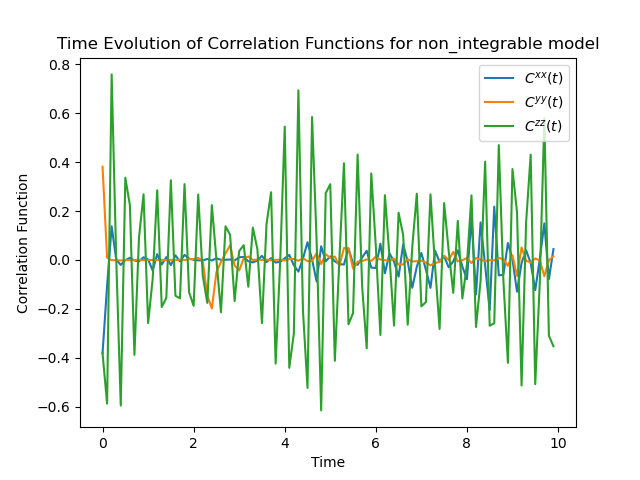
\includegraphics[width=\textwidth]{non_integrable_correlation_functions.png}
        \caption{Non-integrable model}
    \end{subfigure}
    \hfill
    \begin{subfigure}[b]{0.4\textwidth}
        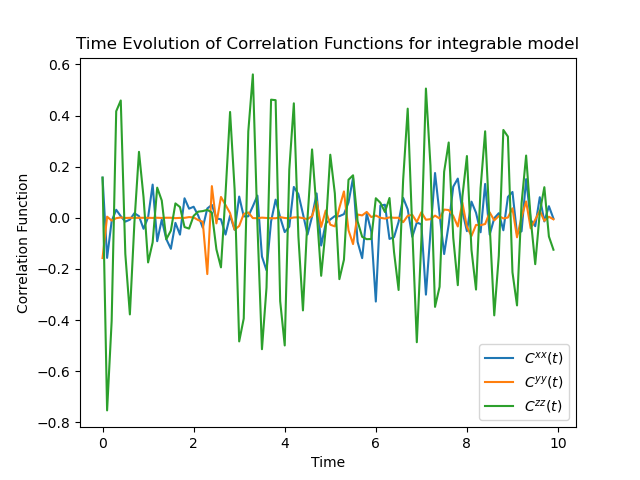
\includegraphics[width=\textwidth]{integrable_correlation_functions.png}
        \caption{Integrable model}
    \end{subfigure}
    \caption{Correlation functions for different models}
\end{figure}
% Inline Python code in the document
\begin{lstlisting}[language=Python]
import numpy as np
import matplotlib.pyplot as plt
from hw4.src.p4_1.imaginary_tebd_fns import create_trotter_gates, create_initial_mps, imaginary_tebd_step
from hw4.src.p4_3.dynamics_fns import real_tebd_step, plot_correlation_functions
from hw4.src.contraction_fns import apply_local_hamiltonian, compute_contraction
L = 12
total_time = 10
dt = 0.1
times = np.arange(0, total_time, dt)
initial_state = create_initial_mps(L, 'neel')
chi_values = [16]
conv_tol = 1e-6

for model in ['non_integrable', 'integrable']:
    if model == 'non_integrable':
        h_z_val = 0.5
    elif model == 'integrable':
        h_z_val = 0.0
    # first we want to do an imagine time tebd two find the ground state
    gate_field, gate_odd, gate_even = create_trotter_gates(1j*dt, h_z=h_z_val)
    
    for time in times:
        state = imaginary_tebd_step(initial_state, chi_values[0], time, [gate_field, gate_odd, gate_even])
        # compute the energy of the state
        energy = apply_local_hamiltonian(state, h_z=h_z_val)
        print(f'Energy at time {time} is {energy}')
        if time > 0:
            if np.abs(energy - previous_energy) / np.abs(energy) < conv_tol:
                gs = state
                break
        # set the values equal to the value from the previous alteration
        previous_energy = energy
        initial_state = state    
    
    # Now, use real-time TEBD to calculate the correlation functions
    # we must create new gates first
    gate_field, gate_odd, gate_even = create_trotter_gates(-dt, h_z=h_z_val)
    correlation_functionS_time_evolution = {}
    for coordinate in ['x', 'y', 'z']:
        bra = gs
        ket = gs

        correlation_function_time_evolution = {}

        for time in times:
            for braket in ['bra', 'ket']:
                if braket == 'bra':
                    transformed_bra = real_tebd_step(bra, chi_values[0], time, braket, [gate_field, gate_odd, gate_even], coordinate)
                    bra = transformed_bra
                if braket == 'ket':
                    transformed_ket = real_tebd_step(ket, chi_values[0], time, braket, [gate_field, gate_odd, gate_even], coordinate)
                    ket = transformed_ket
            correlation_function_time_evolution[time] = compute_contraction(transformed_bra, transformed_ket)


        correlation_functionS_time_evolution[coordinate] = correlation_function_time_evolution

    plot_correlation_functions(correlation_functionS_time_evolution, model)
        





def real_tebd_step(current_mps, chi, time, braket, gates, coordinate):
    """Real time evolution using TEBD."""
    gate_field, gate_odd, gate_even = gates
    transformed_state = []
    if braket == 'ket':
        transformed_state = apply_observable(current_mps.copy(), coordinate)
    trotterized = apply_trotter_gates(current_mps, gate_field, gate_odd, gate_even)
    mps_enforced = enforce_bond_dimension(trotterized, chi)
    if braket == 'bra':
        transformed_state = apply_observable(mps_enforced.copy(), coordinate)
    return transformed_statedef plot_correlation_functions(correlation_functionS_time_evolution, model):
    plt.figure()
    times = sorted(next(iter(correlation_functionS_time_evolution.values())).keys())
    coordinates = ['x', 'y', 'z']
    labels = {'x': r'$C^{xx}(t)$', 'y': r'$C^{yy}(t)$', 'z': r'$C^{zz}(t)$'}

    for coordinate in coordinates:
        values = [correlation_functionS_time_evolution[coordinate][time] for time in times]
        plt.plot(times, values, label=labels[coordinate])

    plt.xlabel('Time')
    plt.ylabel('Correlation Function')
    plt.title(f'Time Evolution of Correlation Functions for {model} model')
    plt.legend()
    plt.savefig(f'hw4/docs/images/{model}_correlation_functions.png')
\end{lstlisting}

On the other hand, if you were to repeat this calculation for the integrable Ising chain $\left(h_{z}=0\right)$ in the gapped phase, you would find qualitatively different decay for $C^{zz}(t)$ and $C^{xx}(t)$. Repeat the experiment for this case and comment on the behavior of the time decay of correlations for integrable systems. \textbf{I did not see a difference, likely due to the low system size that I was able to reach.}˙
% Inline Python code in the document
\begin{lstlisting}[language=Python]
for model in ['non_integrable', 'integrable']:
    if model == 'non_integrable':
        h_z_val = 0.5
    elif model == 'integrable':
        h_z_val = 0.0
    # first we want to do an imagine time tebd two find the ground state
    gate_field, gate_odd, gate_even = create_trotter_gates(1j*dt, h_z=h_z_val)
...
\end{lstlisting}
\footnotetext{${ }^{1}$ Bardarson, Pollmann, and Moore, PRL 109, 017202 (2012).
}


\end{document}